\documentclass[letterpaper,twoside,11pt]{scrartcl}
\usepackage{geometry}
\usepackage[T1]{fontenc}
\usepackage{lmodern}
\usepackage{amssymb,amsmath}
\usepackage{ifxetex,ifluatex}
\usepackage{fixltx2e} % provides \textsubscript
\usepackage{booktabs}
\usepackage{lipsum}
\usepackage{yfonts}
\usepackage{multicol}
\usepackage{librebaskerville}
\usepackage[usenames, dvipsnames]{color}
\usepackage{wrapfig}
\usepackage{tocloft}
\usepackage{tcolorbox}
\usepackage{framed}
\usepackage[headsepline=true, footsepline=false]{scrlayer-scrpage}
\usepackage{letltxmacro}
\usepackage{titlesec}
\usepackage[labelsep=space]{caption}

\definecolor{mygray}{gray}{0.9}

% define TOC charactereistics
\setlength{\cftbeforesecskip}{7px}
\renewcommand{\cftsecdotsep}{3}

% define the page dimensions and margins
\geometry{
papersize={8.5in,11in},
left=.5in,
top=1in,
textwidth=7.5in
}
\headsep = .25in

% adjust section numbering (disable)
\setcounter{secnumdepth}{-2}

% adjust section header spacing and lines
\newcommand{\sectionfont}{\Large\bfseries}
\titlespacing{\section}{0pt}{\parskip}{-\parskip}
\titleformat{\section}
    {\titlerule     
     \vspace{0.25ex}%
     \sectionfont}
    {\thesection}{1em}
    {\sectionfont}[\vspace{0.25ex}%
     \sectionfont
     \titlerule
     \vspace{0.25ex}%
     \sectionfont]


% Define column definitions
\setlength{\columnsep}{.25in}

\usepackage{graphicx}

% Header and footer definitions
%\clearpairofpagestyles
\lohead{Bits \& Bites}
\rohead{ }
\rehead{Bits \& Bites}
\lehead{ }
%\chead{\pagemark}
%\ihead{Title description}

\renewcommand*\pagemark{{\usekomafont{pagenumber}Page\nobreakspace\thepage}}
\addtokomafont{pageheadfoot}{\upshape}

%==============================================================================
% Modify the includegraphics command to be wrapped in wrapfigure ==============
\let\originalincludegraphics\includegraphics
\LetLtxMacro{\newincludegraphics}{\includegraphics}
\renewcommand{\includegraphics}[2][\newincludegraphics]%
    {\begin{wrapfigure}{l}{1.0in}
    \newincludegraphics[{#1}]{#2}
    \end{wrapfigure}
}

%===============================================================================

%\captionsetup{labelformat=empty}
\renewcommand{\figurename}{}
\renewcommand{\thefigure}{}
 

%==============================================================================
% Title Stuff  ================================================================

\def\paperslogan{``Where Can I Find \& Share Data?''}
\def\papername{Bits \& Bites}
\def\paperlocation{Albuquerque, NM}

\renewcommand{\maketitle}{
\vspace*{-40pt}
\begin{center}
\originalincludegraphics[width=3in]{ullogo.png}
\hfill{\Huge\usefont{T1}{ptm}{b}{it} \papername}\\
%\vspace*{0.15in}
\rule[2pt]{\textwidth}{0.25pt}\\
\paperslogan\\
\rule[2pt]{\textwidth}{0.5pt}\\
{\small VOL.  No.  \hfill April 27, 2018}\\
\rule[6pt]{\textwidth}{1.2pt}
\end{center}
}
%==============================================================================

\providecommand{\tightlist}{%
  \setlength{\itemsep}{0pt}\setlength{\parskip}{0pt}}

%==============================================================================
% Deal with longtable issue in multicolumn documents
% from: http://tex.stackexchange.com/questions/161431/how-to-solve-longtable-is-not-in-1-column-mode-error/224096#224096
%\makeatletter
%\let\oldlt\longtable
%\let\endoldlt\endlongtable
%\def\longtable{\@ifnextchar[\longtable@i \longtable@ii}
%\def\longtable@i[#1]{\begin{figure}[t]
%\onecolumn
%\begin{minipage}{0.5\textwidth}
%\oldlt[#1]
%}
%\def\longtable@ii{\begin{figure}[t]
%\onecolumn
%\begin{minipage}{0.5\textwidth}
%\oldlt
%}
%\def\endlongtable{\endoldlt
%\end{minipage}
%\twocolumn
%\end{figure}}
%\makeatother
%==============================================================================



% use upquote if available, for straight quotes in verbatim environments
\IfFileExists{upquote.sty}{\usepackage{upquote}}{}
\ifnum 0\ifxetex 1\fi\ifluatex 1\fi=0 % if pdftex
  \usepackage[utf8]{inputenc}
\else % if luatex or xelatex
  \ifxetex
    \usepackage{mathspec}
    \usepackage{xltxtra,xunicode}
  \else
    \usepackage{fontspec}
  \fi
  \defaultfontfeatures{Mapping=tex-text,Scale=MatchLowercase}
  \newcommand{\euro}{€}
    \setmainfont{CormorantGaramond}
    \setsansfont{merriweather}
\fi
% use microtype if available
\IfFileExists{microtype.sty}{\usepackage{microtype}}{}

\ifxetex
  \usepackage[setpagesize=false, % page size defined by xetex
              unicode=false, % unicode breaks when used with xetex
              xetex]{hyperref}
\else
  \usepackage[unicode=true]{hyperref}
\fi
\hypersetup{breaklinks=true,
            bookmarks=true,
            pdfauthor={Jonathan Wheeler \& Karl Benedict},
            pdftitle={Bits \& Bites},
            colorlinks=true,
            citecolor=blue,
            urlcolor=blue,
            linkcolor=magenta,
            pdfborder={0 0 0}}
\urlstyle{same}  % don't use monospace font for urls

\setlength{\parindent}{0pt}
\setlength{\parskip}{6pt plus 2pt minus 1pt}
\setlength{\emergencystretch}{3em}  % prevent overfull lines


\title{Bits \& Bites}
\subtitle{Where Can I Find \& Share Data?}
\author{Jonathan Wheeler \& Karl Benedict}
\date{April 27, 2018}

\begin{document}

\pagestyle{headings}

\thispagestyle{empty}
\maketitle

\begin{tcolorbox}[colback=blue!5,colframe=red!75!black,title=Announcements] 

\end{tcolorbox}

\begin{multicols}{2}


\section{Repositories: Open Data
Infrastructure}\label{repositories-open-data-infrastructure}

\subsection{Open Data: Why?}\label{open-data-why}

Policies and drivers include federal and other funder requirements:

\begin{itemize}
\tightlist
\item
  White House Office of Science and Technology Policy memo,
  \href{https://obamawhitehouse.archives.gov/blog/2013/02/22/expanding-public-access-results-federally-funded-research}{\emph{Expanding
  Public Access to the Results of Federally Funded Research}}\footnote{White
    House Office of Science and Technology Policy (OTSP) (2013).
    \emph{Expanding Public Access to the Results of Federally Funded
    Research.}
    \url{https://obamawhitehouse.archives.gov/blog/2013/02/22/expanding-public-access-results-federally-funded-research}}
\item
  \href{https://www.gatesfoundation.org/how-we-work/general-information/open-access-policy}{Gates
  Foundation Open Access Policy}\footnote{Bill and Melinda Gates
    Foundation. \emph{Open Access Policy}.
    \url{https://www.gatesfoundation.org/how-we-work/general-information/open-access-policy}}
\end{itemize}

The list goes on - NSF, NIH, DoE, DoD\ldots{}

Policy (sticks) aside, there is likewise research into the cultural,
scientific, and social benefits of making data open and reusable
(carrots). The \href{https://www.nature.com/articles/sdata201618}{Fair
Guiding Principles}\footnote{Nature Scientific Data (2016). The FAIR
  Guiding Principles for scientific data management and stewardship.
  \url{https://www.nature.com/articles/sdata201618}} provide a nice
overview as well as a pretty useful acronym of what \emph{open} means
regarding data:

\textbf{F}indable \textbf{A}ccessible \textbf{I}nteroperable
\textbf{R}eusable

We note the NSF is currently funding projects around research and data
re-use.

\subsection{Classes of Repositories}\label{classes-of-repositories}

Repositories may be categorized in a number of different ways, depending
upon needs:

Compliance with standards that define trustworthyness, measures of
reliability, or other predefined characteristics, such as the

\begin{itemize}
\tightlist
\item
  \href{http://www.crl.edu/sites/default/files/d6/attachments/pages/trac_0.pdf}{Trusted
  Digital Repository (TDR) Checklist}\footnote{RLG-NARA Task Force on
    Digital Repository and Certification (2007). \emph{Trustworthy
    Repositories Audit \& Certification: Criteria and Checklist}.
    Version 1, February 2007. Robin L. Dale and Bruce Ambacher, ed. The
    Center for Research Libraries \& OCLC Online Computer Library
    Center, Inc.
    \url{http://www.crl.edu/sites/default/files/d6/attachments/pages/trac_0.pdf}},
  or its successor
\item
  Trustworthy Digital Repositories -
  \href{https://www.iso.org/standard/56510.html}{ISO 16363}\footnote{International
    Organization for Standardization (ISO) (2012). \emph{ISO 16363:2012
    (CCSDS 652.0-R-1) Space data and information transfer systems --
    Audit and certification of trustworthy digital repositories}.
    \url{https://www.iso.org/standard/56510.html}}/\href{https://public.ccsds.org/pubs/652x0m1.pdf}{CCSDS
  652.0-M-1}\footnote{The Consultative Committee for Space Data Systems
    (2011). \emph{Audit and Certification of Trustworthy Digital
    Repositories Recommended Practice} CCSCS 652.0-M-1.
    \url{https://public.ccsds.org/pubs/652x0m1.pdf}}
\item
  \href{https://www.datasealofapproval.org/en/}{Data Seal of
  Approval}\footnote{Data Seal of Approval website (2018).
    \url{https://www.datasealofapproval.org/en/}}
\end{itemize}

\begin{figure}
\centering

\includegraphics[width=3.50000in]{Digitalrepositorystandards.png}
\caption{Diagram illustrating the development of digital repositories
standards}
\end{figure}

Types of content that those repositories focus on:

\begin{itemize}
\tightlist
\item
  \textbf{Disciplinary repositories} that specialize in content produced
  by specific research disciplines such as
  \href{https://www.icpsr.umich.edu/icpsrweb/landing.jsp}{ICPSR}\footnote{Inter-University
    Consortium for Political and Social Research (ICPSR).
    \url{https://www.icpsr.umich.edu/icpsrweb/landing.jsp}} for social
  science data, the
  \href{http://archaeologydataservice.ac.uk/}{Archaeology Data
  Service}\footnote{Archaeology Data Service (ADS).
    \url{http://archaeologydataservice.ac.uk/}} for archaeological data,
  and \href{http://www.ncbi.nlm.nih.gov/genbank/}{GenBank}\footnote{GenBank.
    \url{http://www.ncbi.nlm.nih.gov/genbank/}} for genetic sequence
  data.
\item
  \textbf{General or Interdisciplinary repositories} that contain
  content that cross disciplinary boundaries, and may also contain
  multiple types of content including data, documents, and multi-media
  files.
\end{itemize}

Or, the organizations that host/manage the repositories - frequently as
a designated repository for data products produced by or with funds from
those organizations. For example:

\begin{itemize}
\tightlist
\item
  \href{https://catalog.data.gov/dataset}{Data.gov}\footnote{Data.gov
    (2018). \url{https://catalog.data.gov/dataset}} - the discovery
  portal for data generated and provided by US Federal Government
  agencies, and some states, municipalities, and universities
\item
  NASA's \href{https://earthdata.nasa.gov/about/daacs}{Distributed
  Active Archive Centers (DAACS)}\footnote{NASA Distributed Active
    Archive Centers (DAACS) (2018).
    \url{https://earthdata.nasa.gov/about/daacs}} - the 12 distributed
  data centers supported by NASA that provide discovery and access to
  different thematic collections of Earth science data.
\item
  UNM's \href{http://digitalrepository.unm.edu}{digital
  repository}\footnote{UNM's Institutional Repository (2018).
    \url{http://digitalrepository.unm.edu}} - the designated
  \emph{institutional repository} for the University of New Mexico.
\end{itemize}

\subsection{Open Data: Where?}\label{open-data-where}

Requirements for repository services will vary from case to case, and
there is no one-size-fits-all solution. Relevant factors include:

\begin{itemize}
\tightlist
\item
  Trusted repository status
\item
  Capacity and commitment to preservation
\item
  Provision of permanent identifiers (DOI)
\item
  Format support
\item
  Federation, discovery, and interoperability with other systems
\end{itemize}

Often these and other repository characteristics and policies are
documented. Resources for identifying and assessing repositories
include:

\begin{itemize}
\tightlist
\item
  PLOS ONE Data Availability policy (includes a
  \href{http://journals.plos.org/plosone/s/data-availability}{list of
  recommended repositories}\footnote{PLOS ONE (2014). \emph{Data
    Availability.}
    \url{http://journals.plos.org/plosone/s/data-availability}})
\item
  Nature Scientific Data
  \href{https://www.nature.com/sdata/policies/repositories}{Recommended
  Data Repositories}\footnote{Nature Scientific Data (2018).
    \emph{Recommended Data Repositories.}
    \url{https://www.nature.com/sdata/policies/repositories}}
\item
  Scientific Data
  \href{https://figshare.com/articles/Scientific_Data_recommended_repositories_June_2015/1434640}{recommended
  repositories}\footnote{Scientific Data (2018). \emph{Scientific Data
    Recommended Repositories.}
    \href{https://figshare.com/articles/Scientific_Data_recommended_repositories_June_2015/1434640}{doi:10.6084/m9.figshare.1434640.v11}}
\item
  Registry of Research Data Repositories
  \href{https://www.re3data.org/}{(re3data.org)}\footnote{Registry of
    Research Data Repositories (2018). \url{https://www.re3data.org/}}
\end{itemize}

\subsection{A Synthesis}\label{a-synthesis}

\begin{figure}
\centering
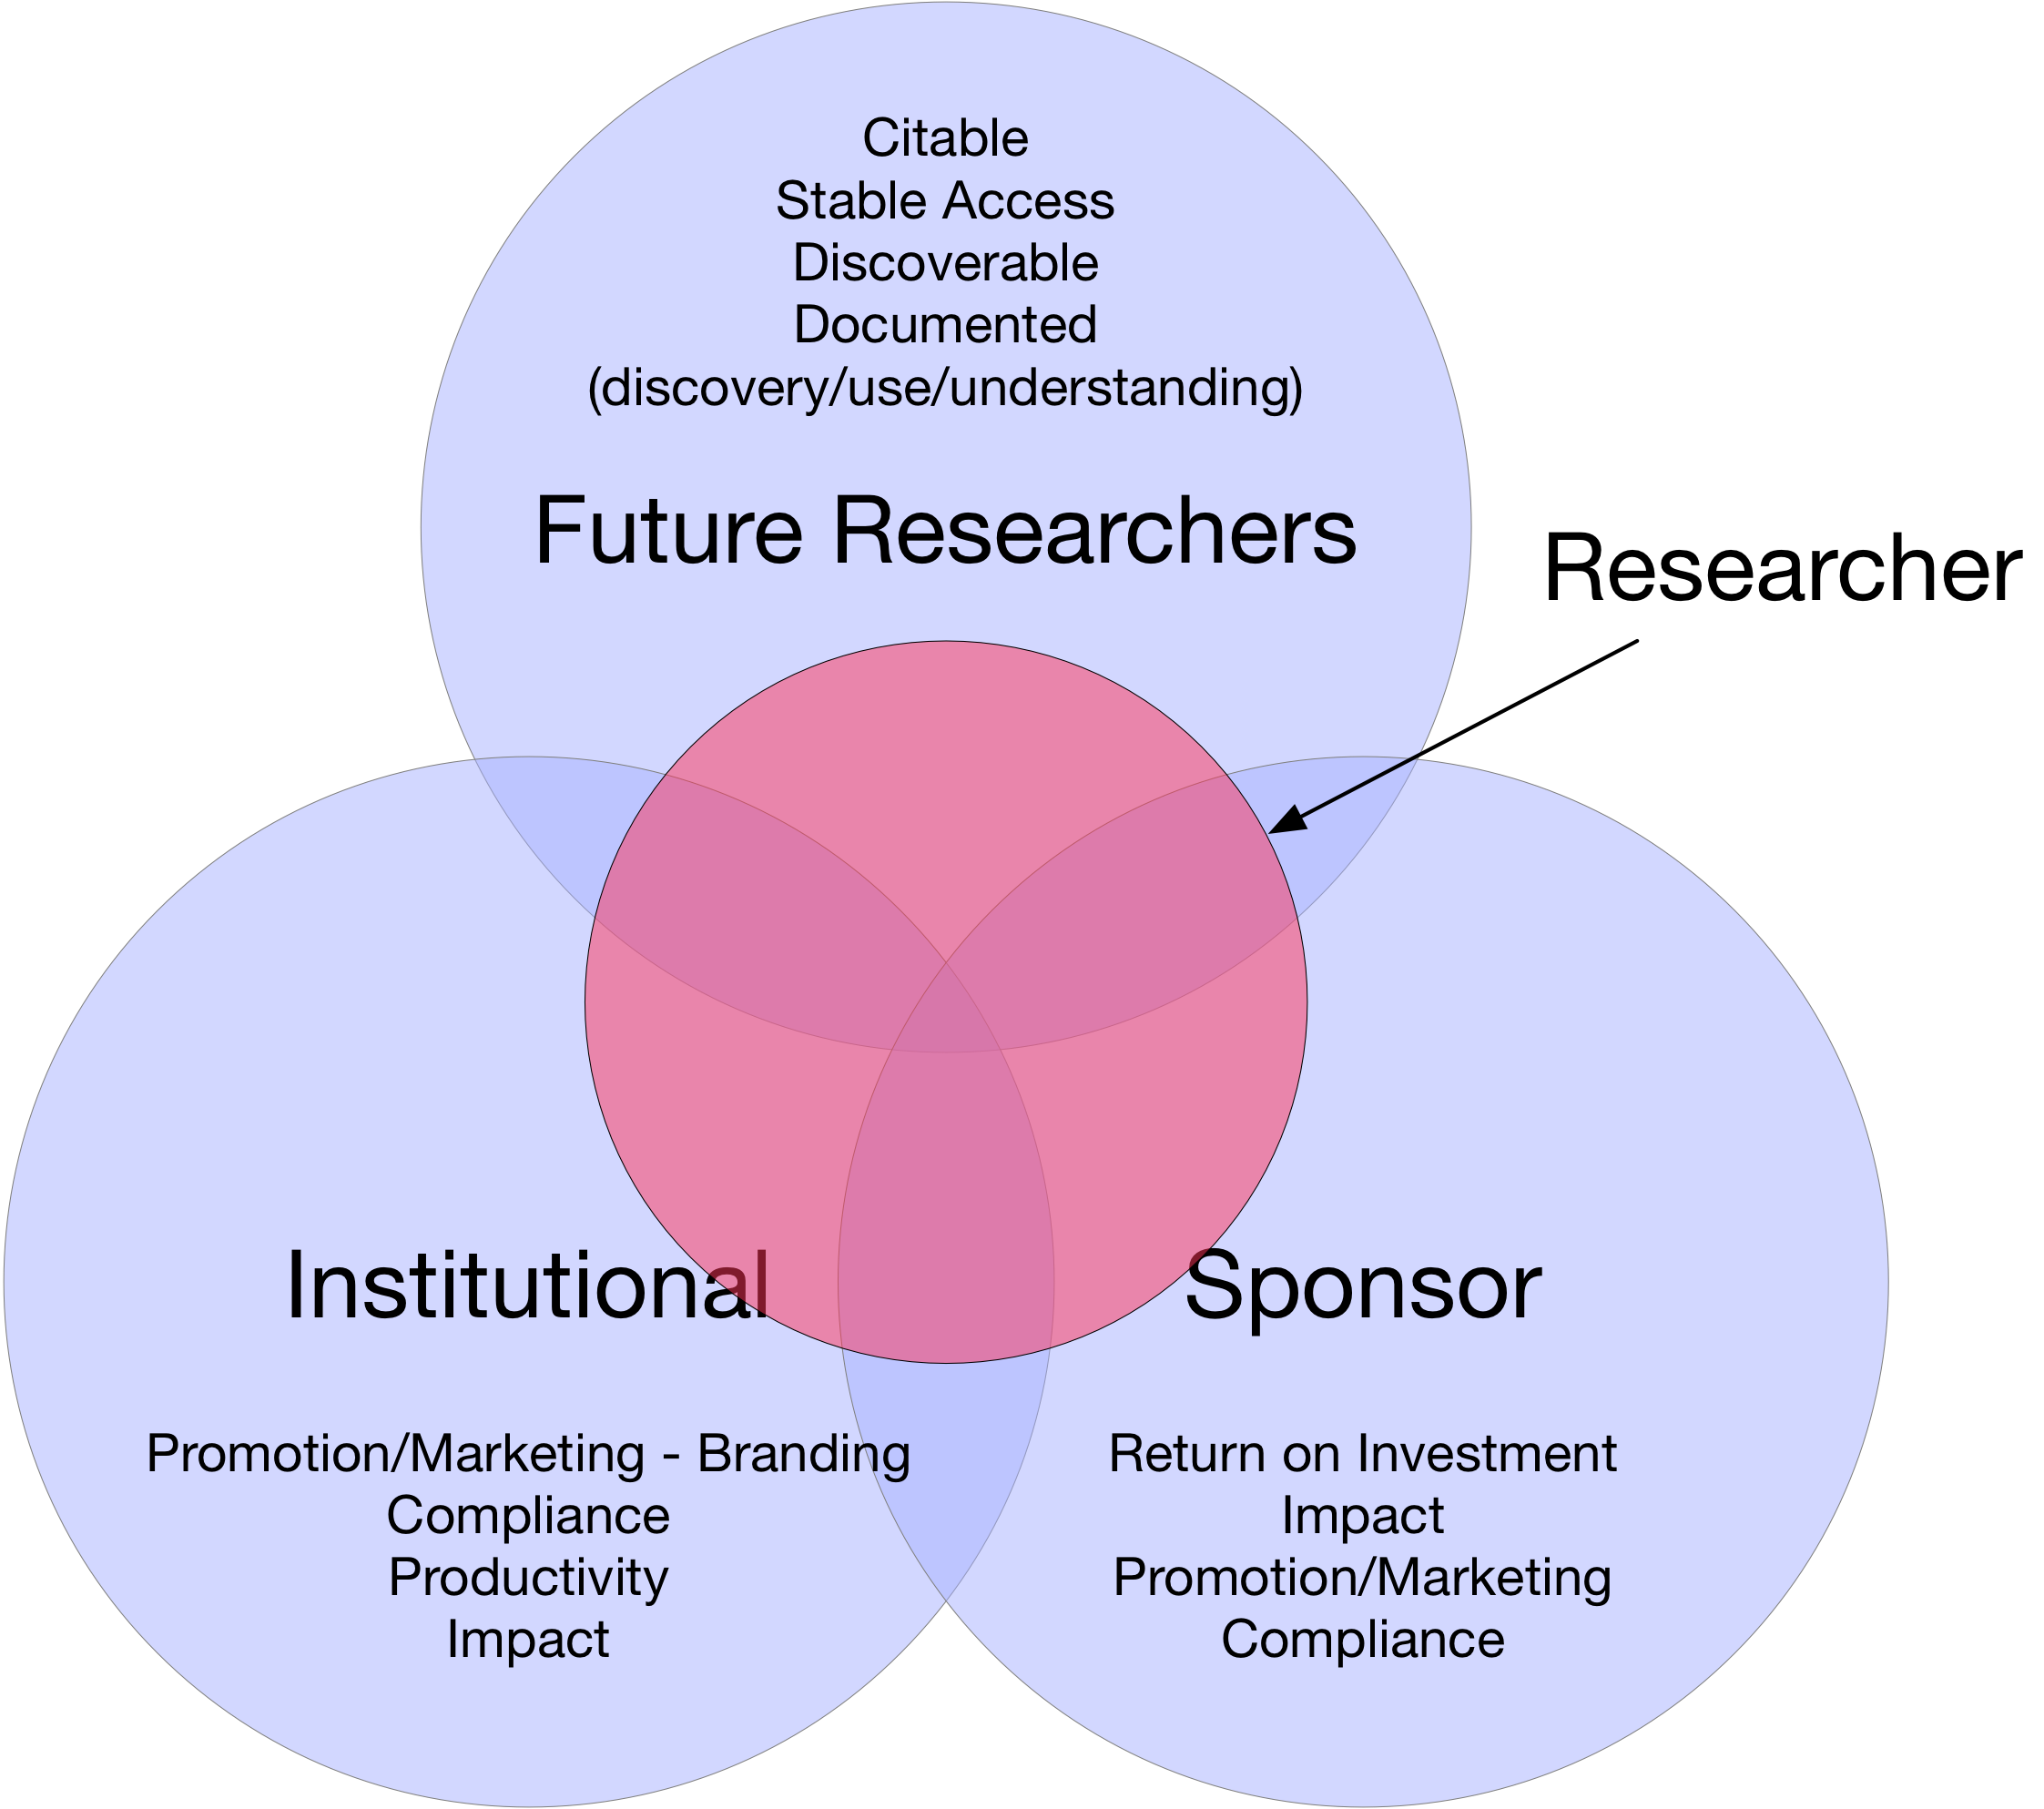
\includegraphics[width=3.50000in]{Venn.png}
\caption{Intersecting Interests}
\end{figure}

\begin{center}\rule{0.5\linewidth}{\linethickness}\end{center}

\section{Further Reading}\label{further-reading}

\begin{itemize}
\tightlist
\item
  Baker, Karen S., and Lynn Yarmey. ``Data Stewardship: Environmental
  Data Curation and a Web-of-Repositories.'' \emph{International Journal
  of Digital Curation} 4, no. 2 (2009): 12-27.
  https://doi.org/10.2218/ijdc.v4i2.90
\item
  Beagrie, Neil, and John Houghton. ``The Value and Impact of Data
  Sharing and Curation: A Synthesis of Three Recent Studies of UK
  Research Data Centres.'' London: JISC, 2014.
  http://repository.jisc.ac.uk/5568/1/iDF308\_-\_Digital\_Infrastructure\_Directions\_Report\%2C\_Jan14\_v1-04.pdf
\end{itemize}

\begin{center}\rule{0.5\linewidth}{\linethickness}\end{center}

Download this document:
\href{https://unmrds.github.io/bb-security/bb-discovery.pdf}{https://unmrds.github.io/bb-discovery/bb-discovery.pdf}\\
Github Repository: \url{https://github.com/unmrds/bb-discovery}

\begin{center}\rule{0.5\linewidth}{\linethickness}\end{center}




\end{multicols}


\end{document}
